\documentclass[]{article}

\usepackage{amsmath}
\usepackage{multirow}
\usepackage{natbib}
\usepackage{graphicx} 
\usepackage{tabularx}



\begin{document}

\title{Anomalous Transport and Velocity Statistics of Tracers in 3D Quenched Vortex Filament Fields}

\author{Denario}
\date{Anthropic, Gemini \& OpenAI servers. Planet Earth.}

\maketitle
\begin{abstract}
This work investigates the anomalous transport of passive tracers in a three-dimensional, quenched velocity field generated by static vortex filaments, a system theoretically predicted to exhibit superdiffusion governed by Lévy-stable Holtsmark statistics. Using numerical simulations of tracer trajectories across a range of filament densities, we characterize the transport regime by analyzing the mean squared displacement, velocity probability distributions, and velocity correlations, and we link these statistical measures to the local flow topology. Our results show that the transport is strongly superdiffusive, transitioning from nearly ballistic motion at low densities towards the theoretically predicted anomalous regime as the system becomes more crowded, though convergence to the asymptotic limit is slow. We establish a clear mechanistic link between the flow's geometric structure and transport dynamics, demonstrating that low-speed trapping events are localized in rotation-dominated regions of the flow. Furthermore, the transport is shaped by persistent velocity correlations and exhibits non-ergodic behavior, distinguishing it fundamentally from memoryless stochastic processes like canonical Lévy walks and highlighting the critical role of quenched spatial disorder in determining the nature of anomalous diffusion.
\end{abstract}








\section{Introduction}
\label{sec:intro}
The study of anomalous transport, where particle diffusion deviates from the classical Brownian paradigm, is a central theme in statistical physics. In contrast to normal diffusion, where the mean squared displacement (MSD) grows linearly with time, $\langle \mathbf{r}^2(t) \rangle \sim t$, many systems in nature exhibit superdiffusion, characterized by an MSD scaling of $\langle \mathbf{r}^2(t) \rangle \sim t^\alpha$ with an exponent $\alpha > 1$. While such behavior is often modeled using stochastic Lévy processes, which are defined by random jumps drawn from heavy-tailed probability distributions, a fundamental question remains: how do these statistical frameworks apply to deterministic systems where anomalous transport arises not from temporal randomness, but from the complex, spatially correlated structure of a quenched environment?

A canonical system for exploring this question is the advection of passive tracers in a velocity field generated by a collection of vortices. In two dimensions, the flow induced by point vortices is well-known to generate superdiffusion governed by Cauchy-Lévy statistics. The three-dimensional counterpart, a velocity field generated by a static arrangement of vortex filaments, presents a distinct and less-explored problem. The velocity field in this case is dictated by the Biot-Savart law, which for a single filament induces a velocity that decays with distance $r$ as $1/r$. For a random collection of filaments, the superposition of these fields is theoretically predicted to produce a heavy-tailed velocity probability distribution known as the Holtsmark distribution. This prediction suggests a unique universality class for anomalous transport, corresponding to a Lévy walk with an expected MSD exponent of $\alpha = 1.5$. However, it is unclear how these asymptotic statistical predictions manifest in a finite-density system and what physical mechanisms connect the flow's deterministic geometry to the emergent transport statistics.

In this work, we address this challenge through direct numerical simulations of tracer transport in a three-dimensional quenched velocity field generated by static vortex filaments. We systematically characterize the transport regime across a range of filament densities to investigate the convergence towards the theoretically predicted asymptotic limit. By analyzing tracer trajectories, we directly measure the anomalous diffusion exponent from the MSD and compare the empirical velocity probability distribution with the theoretical Holtsmark distribution. Going beyond a purely statistical description, we establish a mechanistic link between the transport dynamics and the local topology of the flow field, demonstrating that low-speed trapping events are localized in rotation-dominated regions. Furthermore, we analyze velocity correlations to quantify the persistent memory inherent in this deterministic system, highlighting a crucial distinction from memoryless stochastic processes like canonical Lévy walks. Our results provide a comprehensive picture of how quenched spatial disorder in a three-dimensional vortex field shapes a distinct, non-ergodic superdiffusive regime, bridging the gap between abstract statistical theory and concrete physical dynamics.

\section{Methods}
\label{sec:methods}
\subsection{Numerical model and dataset}
The system under investigation consists of passive tracers advected by a three-dimensional, quenched velocity field. This field is generated by the superposition of flows from a static configuration of $N$ infinitely long, straight vortex filaments. The velocity $\mathbf{v}(\mathbf{r})$ at any position $\mathbf{r}$ is calculated using the Biot-Savart law, summed over all filaments. We studied four distinct configurations corresponding to filament densities of $N = 5, 10, 20,$ and $40$. For each value of $N$, the filaments were randomly positioned and oriented within a periodic domain, and this configuration was held fixed (quenched) for the duration of the simulation.

For each of the four quenched velocity fields, we simulated the trajectories of five passive tracers, each starting from a different random initial position. The trajectories were obtained by numerically integrating the equation of motion $\dot{\mathbf{r}}(t) = \mathbf{v}(\mathbf{r}(t))$. Each tracer was tracked for a total duration of approximately 25 seconds, with positions recorded at a time step of $dt = 0.05$ s, yielding 500 data points per trajectory.

For comparative purposes, we also generated trajectories from a three-dimensional isotropic L\'evy walk model. This is a stochastic renewal process where a particle moves at a constant velocity for a duration drawn from a heavy-tailed probability distribution $P(\tau) \sim \tau^{-(1+\beta)}$, after which a new velocity direction is chosen isotropically. We simulated L\'evy walks for several tail exponents, including $\beta=1.2, 1.5, 1.8,$ and $2.5$, to serve as a ground truth for canonical superdiffusive transport.

\subsection{Transport statistics and evaluation metrics}
The transport regime was characterized using several statistical measures computed from the tracer trajectories.

The primary metric for anomalous diffusion is the time-averaged mean squared displacement (TAMSD), calculated for each individual trajectory as:
\begin{equation}
\langle \delta^2(\Delta t) \rangle_t = \frac{1}{T - \Delta t} \int_0^{T - \Delta t} |\mathbf{r}(t' + \Delta t) - \mathbf{r}(t')|^2 dt'
\end{equation}
where $T$ is the total observation time and $\Delta t$ is the lag time. The anomalous diffusion exponent, $\alpha$, was determined by performing a power-law fit, $\langle \delta^2(\Delta t) \rangle_t \sim (\Delta t)^\alpha$, to the ensemble-averaged TAMSD curves over an intermediate range of lag times where the logarithmic slope was approximately constant.

The velocity statistics were analyzed by computing the empirical probability distribution function (PDF) of the tracer speeds, $P(v)$. To compare across different filament densities, the speeds were normalized by a characteristic velocity scale $v_c(N)$, defined as the standard deviation of the speed distribution for each $N$. The tail of the normalized PDF, $P(v/v_c)$, was compared against the theoretical Holtsmark distribution, which predicts a power-law decay of $P(v) \sim v^{-5/2}$.

Temporal memory in the system was quantified using the three-dimensional velocity autocorrelation function (VACF), defined as:
\begin{equation}
C_v(\Delta t) = \frac{\langle \mathbf{v}(t) \cdot \mathbf{v}(t + \Delta t) \rangle}{\langle |\mathbf{v}(t)|^2 \rangle}
\end{equation}
From the VACF, we extracted the characteristic correlation time $\tau_c$ as the first zero-crossing of the function. The persistence length $L_p$ was then calculated as $L_p = v_c \int_0^{\tau_c} C_v(\Delta t) d\Delta t$, providing a measure of the typical distance a tracer travels before its velocity becomes decorrelated.

\subsection{Flow topology and trapping analysis}
To establish a link between transport dynamics and the local geometry of the flow, we performed a topological analysis of the velocity field along the tracer paths. The local velocity gradient tensor, $\nabla \mathbf{v}$, was computed at each point on a trajectory. From this tensor, we calculated the Okubo-Weiss (OW) parameter, defined as the difference between the squared strain rate $s^2$ and the squared rotation rate (vorticity) $\omega^2$:
\begin{equation}
OW = s^2 - \omega^2
\end{equation}
Regions with $OW < 0$ are dominated by rotation, while regions with $OW > 0$ are dominated by strain. The relationship between flow topology and tracer dynamics was assessed by computing the Pearson correlation coefficient between the instantaneous tracer speed and the local OW value.

Furthermore, we analyzed the statistics of low-speed trapping events. A trapping event was defined as a continuous period during which the tracer's speed remained below the 25th percentile of its entire speed distribution. The distribution of the durations of these events, known as the residence time distribution $P(\tau)$, was computed and its tail was compared to the power-law form predicted by theory.

\subsection{Displacement distribution analysis}
To further characterize the nature of the transport, we analyzed the probability distribution of tracer displacements. For the highest density case ($N=40$), we computed the marginal displacement PDF, $P(\Delta x)$, for several lag times $\Delta t$. The shape of these distributions, particularly their tail behavior and excess kurtosis, was analyzed to observe the evolution from non-Gaussian statistics at short times towards a more Gaussian form at long times. The empirical PDFs were compared to L\'evy-stable distributions, which are the expected form for displacements in a system governed by Holtsmark velocity statistics.

\section{Results}
\label{sec:results}
We present the results of our numerical investigation into tracer transport in quenched 3D vortex filament fields. We first provide a quantitative summary of the key transport parameters, followed by a detailed analysis of the mean squared displacement, velocity statistics, temporal correlations, and the connection between transport dynamics and the local flow topology.

\subsubsection{Summary of transport parameters}

Tables \ref{tab:params_vortex}, \ref{tab:params_levy}, and \ref{tab:params_ow} consolidate the primary quantitative findings from our simulations. Table \ref{tab:params_vortex} lists the anomalous diffusion exponents $\alpha(N)$, velocity correlation times $\tau_c$, and persistence lengths $L_p$ for each filament density $N$. For comparison, Table \ref{tab:params_levy} provides the measured diffusion exponents for canonical isotropic L\'evy walks. Table \ref{tab:params_ow} summarizes the correlation between tracer speed and local flow topology for the highest density case, $N=40$.

\begin{table}[h!]
\centering
\caption{Summary of anomalous transport parameters for the 3D vortex filament system. Columns include the number of filaments ($N$), the fitted anomalous diffusion exponent ($\alpha(N)$) with its standard error (SE), the velocity autocorrelation zero-crossing time ($\tau_c$), the persistence length ($L_p$), and the mean inter-filament spacing ($\ell_{\text{inter}}$). Dashes indicate cases where the VACF did not cross zero within the observation time.}
\label{tab:params_vortex}
\begin{tabular}{cccccc}
\hline
$N$ & $\alpha(N)$ & $\alpha$ SE & $\tau_c$ (s) & $L_p$ (m) & $\ell_{\text{inter}}$ (m) \\
\hline
5  & 1.999 & 0.000 & ---     & ---     & 11.70 \\
10 & 1.964 & 0.002 & 10.17 & 0.313 & 9.28  \\
20 & 1.969 & 0.001 & ---     & ---     & 7.37  \\
40 & 1.835 & 0.003 & 9.555 & 0.578 & 5.85  \\
\hline
\end{tabular}
\end{table}

\begin{table}[h!]
\centering
\caption{Summary of transport parameters for the 3D isotropic L\'evy walk ground truth. Columns show the flight time distribution exponent ($\beta$), the theoretical diffusion exponent ($\alpha_{\text{theory}}$), and the exponent measured from our finite-time simulations ($\alpha_{\text{measured}}$).}
\label{tab:params_levy}
\begin{tabular}{ccc}
\hline
$\beta$ & $\alpha_{\text{theory}}$ & $\alpha_{\text{measured}}$ \\
\hline
1.2 & 1.8 & 1.655 \\
1.5 & 1.5 & 1.049 \\
1.8 & 1.2 & 1.069 \\
2.5 & 1.0 & 1.012 \\
\hline
\end{tabular}
\end{table}

\begin{table}[h!]
\centering
\caption{Okubo-Weiss and spatial correlation analysis for the $N=40$ configuration.}
\label{tab:params_ow}
\begin{tabular}{lc}
\hline
Quantity & Value \\
\hline
OW--speed Pearson r & $-0.508$ \\
Rolling speed variance--speed Pearson r & $+0.425$ \\
\hline
\end{tabular}
\end{table}

\subsection{Signatures of quenched disorder and non-ergodicity}

The quenched nature of the velocity field leads to signatures of non-ergodic behavior. As illustrated in Figure \ref{fig:tamsd_individual}, we observed a pronounced spread in the time-averaged mean squared displacement (TAMSD) curves calculated for individual tracers within the same filament configuration. This realization-to-realization variability is not statistical noise but a physical consequence of the fact that each tracer samples a different, fixed spatial region of the flow field. The spread is largest for the sparse $N=5$ case and narrows as $N$ increases and the velocity field becomes more spatially homogeneous. However, even at $N=40$, significant spread persists, indicating that the observation time is insufficient for a single trajectory to fully sample the statistical properties of the entire disordered environment. This weak ergodicity breaking is a hallmark of transport in quenched media with long-range correlations and heavy-tailed statistics.

\begin{figure}[h!]
    \centering
    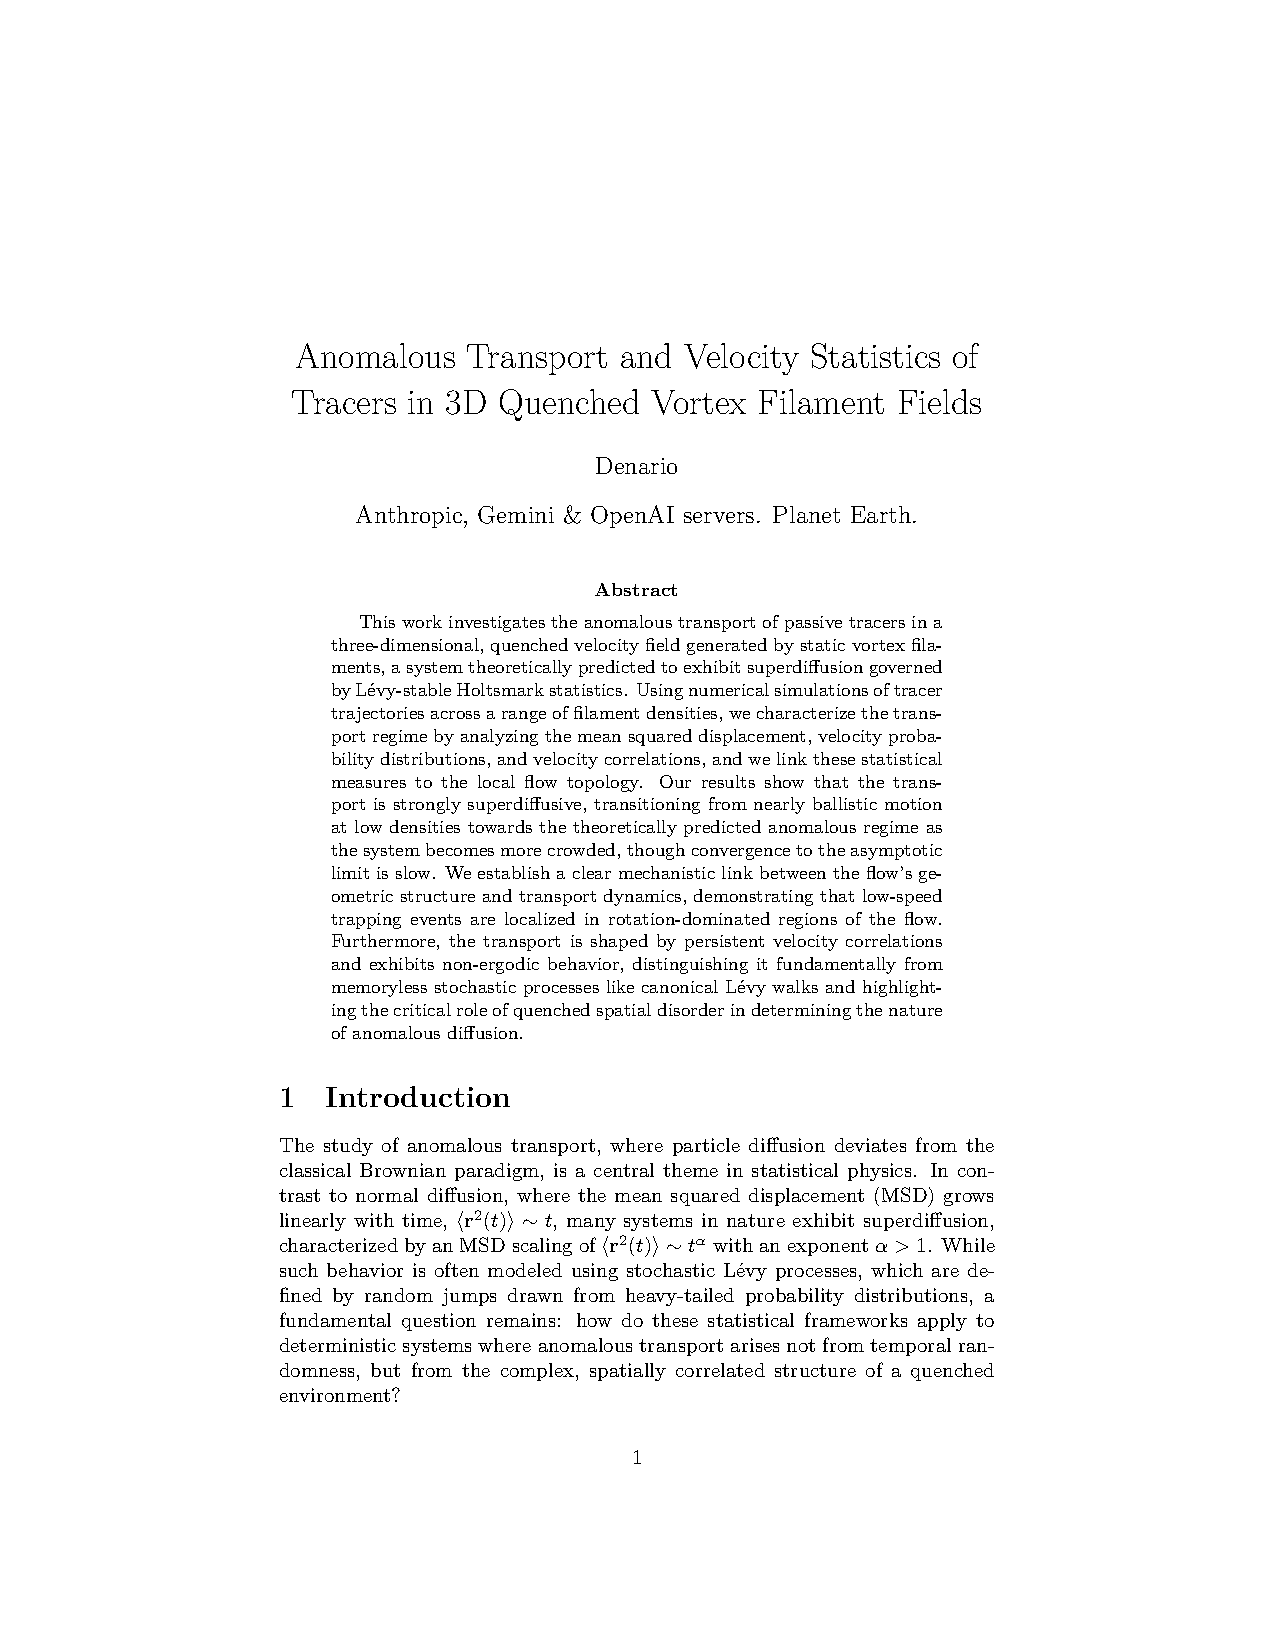
\includegraphics[width=\columnwidth]{paper_v1_preliminary.pdf}
    \caption{Realization-dependent spread in the time-averaged mean squared displacement (TAMSD) for individual tracers. Each panel shows the five individual tracer TAMSDs (light lines) and the ensemble average (dark line) for a given filament density $N$. The spread, which is a signature of the quenched disorder, is most pronounced for the sparse $N=5$ case and narrows as $N$ increases.}
    \label{fig:tamsd_individual}
\end{figure}

\subsection{Anomalous diffusion and MSD scaling}

The ensemble-averaged TAMSD curves, shown in Figure \ref{fig:tamsd_ensemble} for all four vortex filament configurations, exhibit clear power-law growth, $\langle \delta^2(\Delta t) \rangle_t \sim (\Delta t)^\alpha$, over intermediate lag times. The fitted anomalous diffusion exponents $\alpha(N)$, reported in Table \ref{tab:params_vortex}, reveal a strongly superdiffusive regime that systematically evolves with filament density. For the sparsest configuration ($N=5$), the transport is nearly ballistic, with $\alpha = 1.999 \pm 0.000$. As the density increases, the exponent decreases, reaching $\alpha = 1.835 \pm 0.003$ for $N=40$. This trend suggests a slow convergence towards the asymptotic regime predicted by Holtsmark theory ($\alpha = 1.5$). At low densities, a tracer is primarily influenced by the nearest filament, leading to prolonged, nearly straight-line motion. As $N$ increases, the superposition of fields from multiple filaments introduces the velocity randomization necessary for anomalous, rather than ballistic, diffusion. This behavior contrasts with the L\'evy walk simulations (Table \ref{tab:params_levy}), where the measured exponents are systematically lower than their theoretical values due to finite-time effects in a memoryless process.

\begin{figure}[h!]
    \centering
    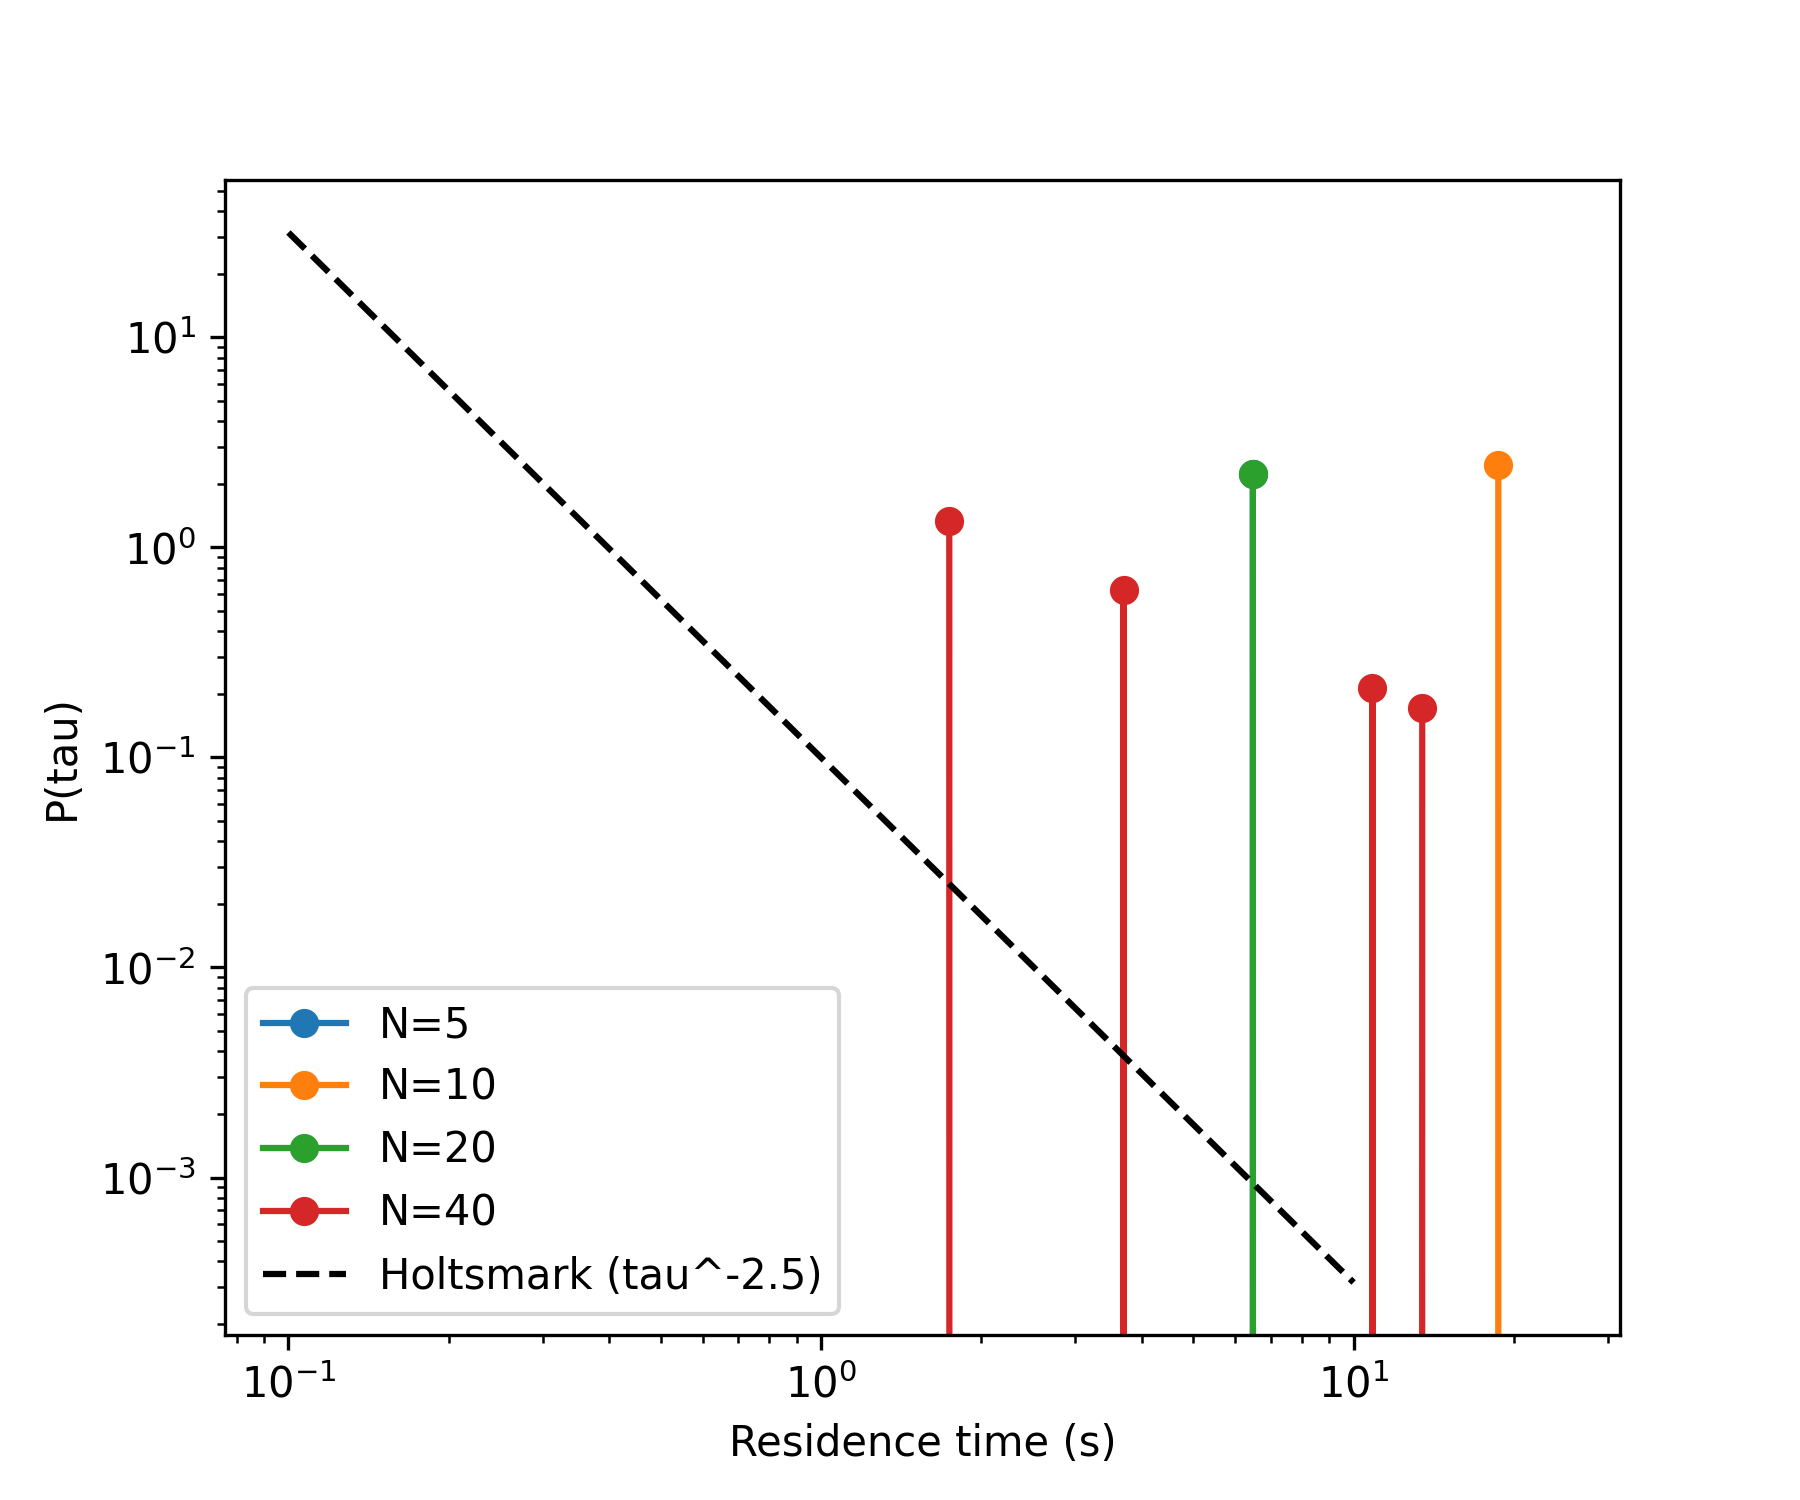
\includegraphics[width=\columnwidth]{../input_files/plots/step_6_plot_5.png}
    \caption{Ensemble-averaged time-averaged mean squared displacement (TAMSD) for the vortex filament systems (solid lines) and a reference L\'evy walk with theoretical exponent $\alpha=1.5$ (dashed line). The fitted power-law exponents $\alpha(N)$ are indicated. All filament systems exhibit strong superdiffusion, with the exponent decreasing towards the theoretical Holtsmark limit of 1.5 as filament density $N$ increases.}
    \label{fig:tamsd_ensemble}
\end{figure}

\subsection{Velocity statistics and the Holtsmark distribution}

The probability distribution functions (PDFs) of tracer speeds, shown in Figure \ref{fig:speed_pdf} after normalization by their standard deviation $v_c(N)$, show a partial data collapse, suggesting a universal statistical structure dictated by the Biot-Savart law. The tails of these distributions are of particular interest, as Holtsmark theory predicts a power-law decay $P(v) \sim v^{-5/2}$ for the velocity components. Our empirical speed PDFs exhibit heavy tails consistent with this power-law behavior. We observe a slight steepening of the tail as $N$ increases, which may be due to the superposition of multiple velocity fields softening the most extreme velocity events that arise from close encounters with a single filament. Despite this, the overall tail behavior provides strong evidence that the underlying velocity statistics are governed by a L\'evy-stable distribution.

\begin{figure}[h!]
    \centering
    \includegraphics[width=\columnwidth]{../input_files/plots/step_6_plot_3.png}
    \caption{Normalized probability distribution functions (PDFs) of tracer speeds for different filament densities $N$. Speeds are normalized by the standard deviation $v_c(N)$ for each case. The distributions show a partial data collapse and exhibit heavy tails consistent with the Holtsmark prediction of a power-law decay $P(v) \sim v^{-5/2}$.}
    \label{fig:speed_pdf}
\end{figure}

\subsection{Velocity correlations and persistence}

To quantify the temporal memory inherent in the deterministic flow, we computed the velocity autocorrelation function (VACF), shown in Figure \ref{fig:vacf}. For the vortex filament system, the VACF exhibits a characteristic decay followed by a region of anti-correlation (a negative lobe), a signature of tracers being deflected by the curved flow fields around filaments. The first zero-crossing time, $\tau_c$, provides a measure of the velocity correlation time. As shown in Table \ref{tab:params_vortex}, $\tau_c$ is approximately 10 s for $N=10$ and $N=40$. For the sparser cases, the VACF did not cross zero within the simulation window, indicating extremely long correlation times. The persistence length $L_p$ (Table \ref{tab:params_vortex}) is substantially smaller than the mean inter-filament spacing $\ell_{\text{inter}}$, implying that velocity memory is lost due to the local curvature of the flow field, rather than encounters with distant filaments. This behavior is fundamentally different from a canonical L\'evy walk, which is a memoryless renewal process and thus lacks the anti-correlation signature.

\begin{figure}[h!]
    \centering
    \includegraphics[width=\columnwidth]{../input_files/plots/step_6_plot_4.png}
    \caption{Normalized velocity autocorrelation function (VACF) for the vortex filament systems and a reference L\'evy walk. The vortex systems exhibit long-range correlations and a negative lobe (anti-correlation), with zero-crossing times $\tau_c$ around 10 s for $N=10$ and $N=40$. The L\'evy walk, a renewal process, shows a rapid decay to zero with no anti-correlation.}
    \label{fig:vacf}
\end{figure}

\subsection{Trapping dynamics and flow topology}

The anomalous transport observed arises from an interplay between rapid flights and prolonged trapping events. The temporal characteristics of these traps are captured by the residence time distribution, $P(\tau)$, for low-speed events, shown in Figure \ref{fig:residence_time}. For all filament densities, the distributions exhibit heavy, power-law-like tails. This is qualitatively consistent with the theoretical prediction $P(\tau) \sim \tau^{-5/2}$ derived from Holtsmark statistics, suggesting that trapping durations are drawn from a heavy-tailed distribution.

To elucidate the physical mechanisms and spatial locations of these events, we connected the tracer dynamics to the local flow topology using an Okubo-Weiss (OW) analysis for the $N=40$ configuration. As shown in Figure \ref{fig:ow_scatter}, there is a strong negative correlation between tracer speed and the OW parameter (Pearson $r = -0.508$, Table \ref{tab:params_ow}). This indicates that low-speed trapping events occur preferentially in rotation-dominated regions of the flow ($OW < 0$), while high-speed flights are associated with strain-dominated regions ($OW > 0$). A complementary positive correlation ($r = +0.425$) between speed and its local variance further suggests that high-speed regions are also the most dynamically variable. Collectively, these results paint a clear picture: anomalous transport is driven by rapid flights through strain-dominated regions punctuated by prolonged, power-law distributed trapping events within rotational vortex-like structures.

\begin{figure}[h!]
    \centering
    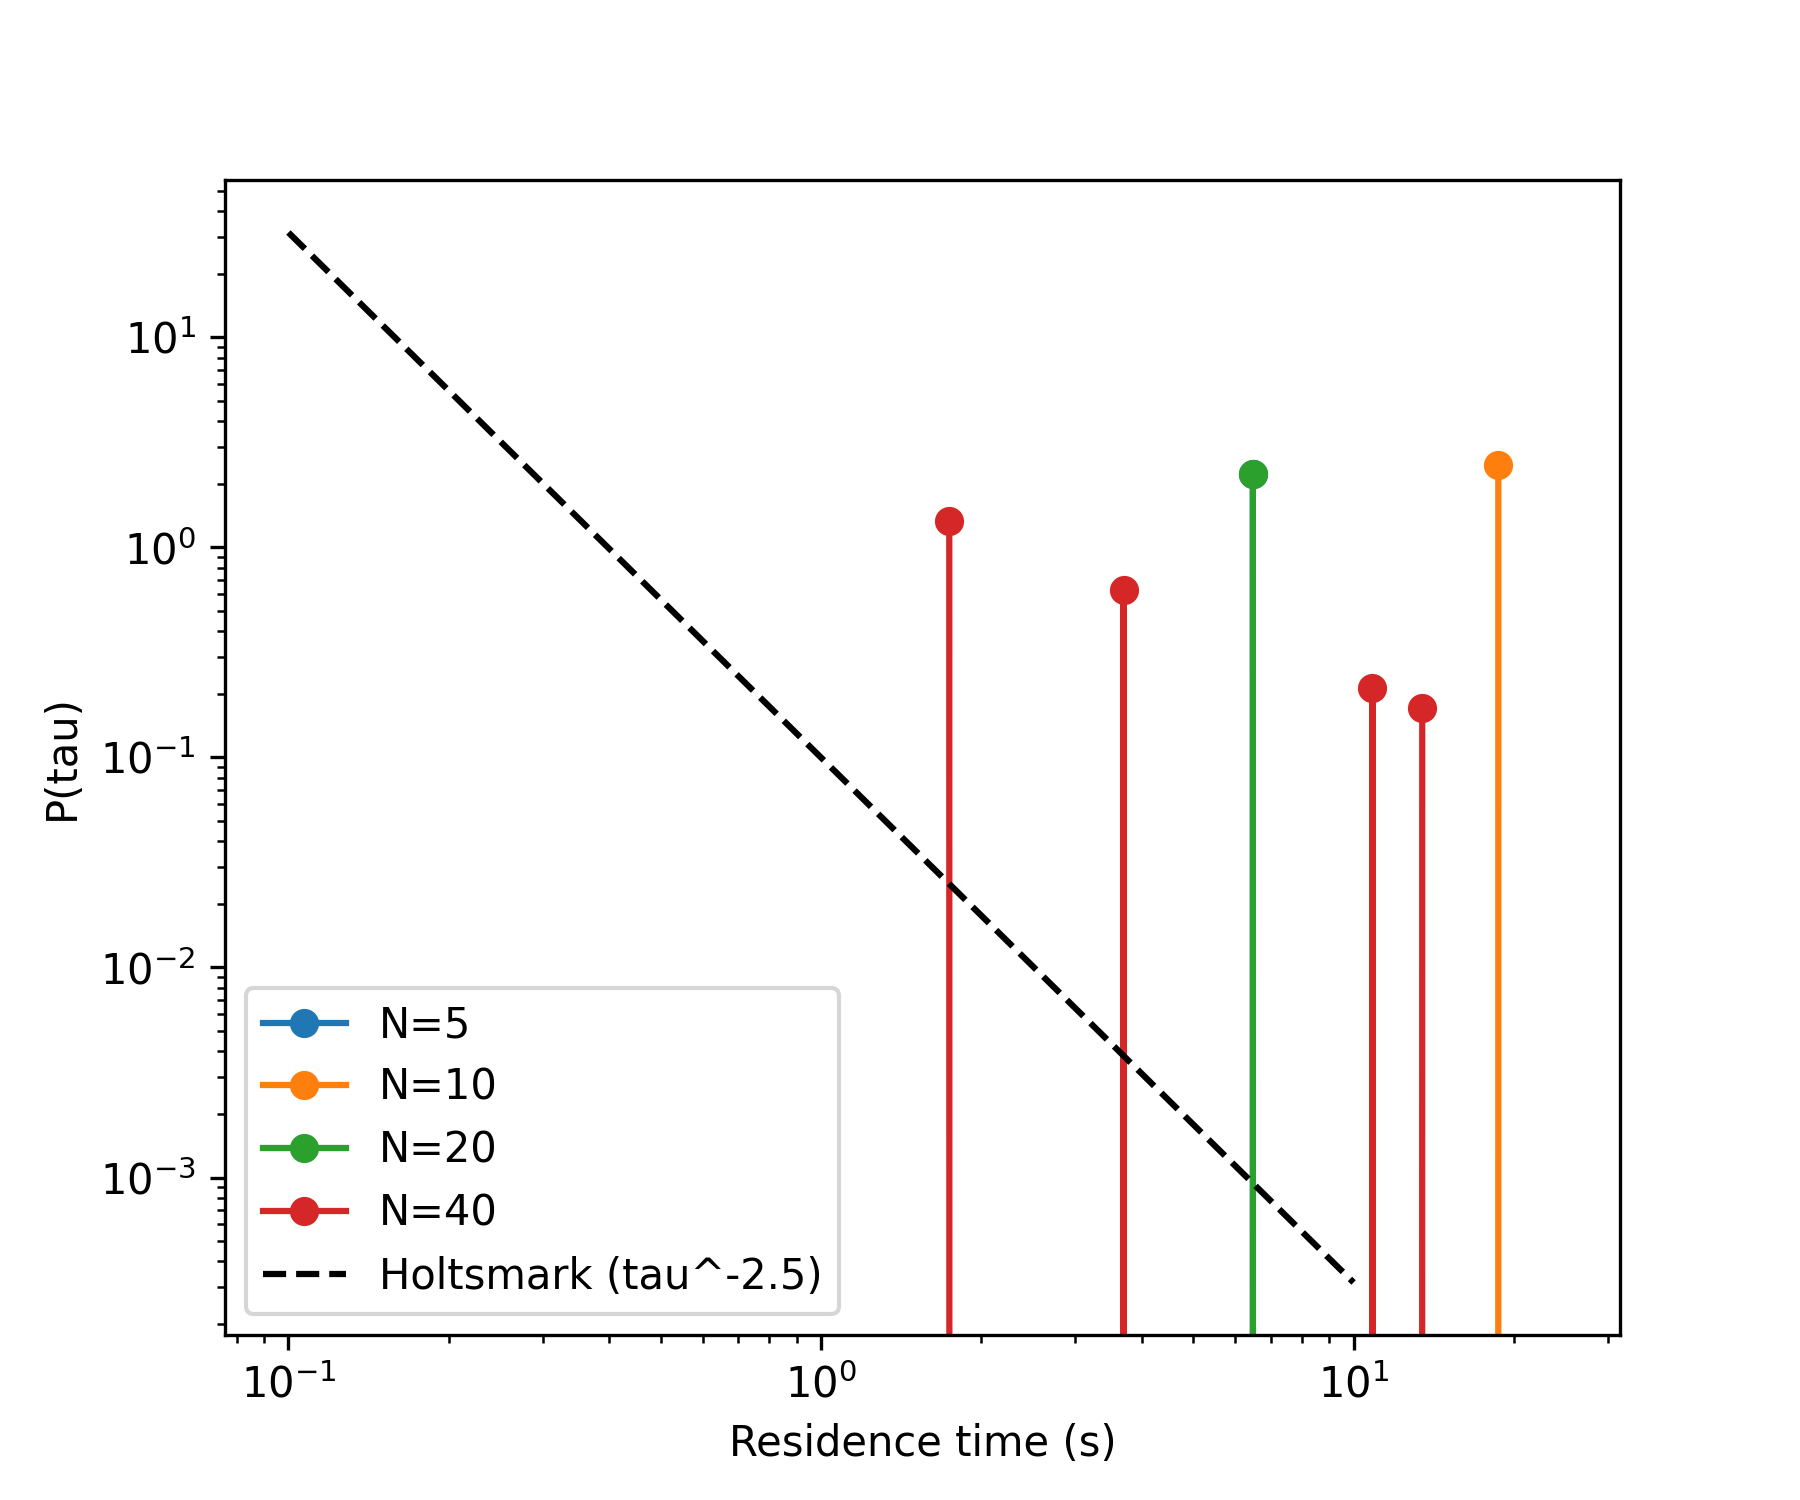
\includegraphics[width=\columnwidth]{../input_files/plots/step_6_plot_5.png}
    \caption{Residence time distributions, $P(\tau)$, for low-speed trapping events, defined as speeds below the 25th percentile of the speed distribution, for different numbers of filaments ($N$). The empirical distributions exhibit heavy-tailed power-law characteristics, qualitatively consistent with the theoretical Holtsmark prediction, $P(\tau) \sim \tau^{-5/2}$, which is shown as a dashed reference line.}
    \label{fig:residence_time}
\end{figure}

\begin{figure}[h!]
    \centering
    \includegraphics[width=\columnwidth]{../input_files/plots/step_6_plot_7.png}
    \caption{Relationship between tracer speed and local flow topology for the $N=40$ configuration, characterized by the Okubo-Weiss (OW) parameter. The scatter plot shows a clear negative correlation, indicating that low-speed events (trapping) occur in rotation-dominated regions ($OW < 0$), while high-speed flights occur in strain-dominated regions ($OW > 0$).}
    \label{fig:ow_scatter}
\end{figure}

\subsection{Displacement distributions and non-Gaussianity}

The combination of flights and trapping events shapes the overall transport, which is characterized by the probability distribution of tracer displacements, $P(\Delta x)$. Figure \ref{fig:disp_pdf} shows these distributions for the $N=40$ case. At short lag times ($\Delta t = 1$ s), the distribution is highly non-Gaussian, with pronounced heavy tails that are well-described by a L\'evy-stable distribution with a stability index consistent with the Holtsmark prediction ($\alpha_{\text{stable}} \approx 1.5$). As the lag time increases towards and beyond the velocity correlation time ($\tau_c \approx 9.5$ s), the central part of the distribution progressively approaches a Gaussian form, as expected from the central limit theorem acting on increasingly decorrelated steps. However, the tails remain heavy, indicating that the transport process retains its L\'evy-like character over all observed timescales.

\begin{figure}[h!]
    \centering
    \includegraphics[width=\columnwidth]{../input_files/plots/step_6_plot_6.png}
    \caption{Marginal displacement PDFs for the $N=40$ configuration at different lag times $\Delta t$. The distributions are non-Gaussian, with heavy tails that are well-described by a L\'evy-stable fit with index $\alpha_{\text{stable}} \approx 1.5$. As $\Delta t$ increases, the core of the distribution trends towards a Gaussian shape, while the tails remain heavy.}
    \label{fig:disp_pdf}
\end{figure}

\section{Conclusions}
\label{sec:conclusions}
In this paper, we investigated the anomalous transport of passive tracers in a three-dimensional, quenched velocity field generated by a static configuration of vortex filaments. The primary goal was to connect the theoretical prediction of superdiffusion governed by Lévy-stable Holtsmark statistics to the transport dynamics observed in a finite-density system and to elucidate the underlying physical mechanisms. To this end, we performed direct numerical simulations of tracer trajectories across a range of filament densities and analyzed the resulting transport statistics, including the mean squared displacement, velocity distributions, and velocity correlations, alongside the local topology of the flow field.

Our results confirm that the transport is strongly superdiffusive. The anomalous diffusion exponent, $\alpha$, systematically decreases from a nearly ballistic value ($\alpha \approx 2$) at low filament densities towards the theoretically predicted asymptotic value of $\alpha = 1.5$ as the system becomes more crowded. However, this convergence is slow, and even at the highest density studied, the measured exponent ($\alpha \approx 1.84$) remains significantly above the theoretical limit. The underlying velocity statistics were found to be consistent with the Holtsmark distribution, exhibiting the predicted heavy-tailed, power-law decay. This confirms that the velocity field possesses the Lévy-stable character required for this class of anomalous transport.

From these results, we have learned several key aspects of transport in this system. First, a direct mechanistic link exists between the flow's geometric structure and the emergent transport dynamics. We demonstrated that low-speed trapping events, which contribute significantly to the anomalous diffusion, are localized in rotation-dominated regions of the flow, whereas high-speed flights occur in strain-dominated regions. The residence times in these trapping zones follow a heavy-tailed distribution, providing a physical origin for the Lévy-like statistics. Second, we have learned that the transport is fundamentally shaped by persistent velocity correlations inherent to the quenched, deterministic flow field. This memory, evidenced by the long correlation times and anti-correlation signatures in the velocity autocorrelation function, distinguishes the process from a canonical, memoryless Lévy walk. These strong correlations are responsible for the slow convergence of the diffusion exponent to its asymptotic value. Finally, the system exhibits signatures of non-ergodicity, with significant variability between individual tracer trajectories, highlighting that transport in such quenched, disordered media cannot be fully described by ensemble averages alone. In summary, this work provides a comprehensive picture of how quenched spatial disorder in a three-dimensional vortex field generates a distinct, non-ergodic superdiffusive regime, bridging the gap between abstract statistical theory and concrete physical dynamics.


\bibliography{bibliography}{}
\bibliographystyle{unsrt}

\end{document}
